% !TEX program = XeLaTeX
% !TEX encoding = UTF-8
\documentclass[UTF8,nofonts]{ctexart}%{article}


\setCJKmainfont[BoldFont=FandolSong-Bold.otf,ItalicFont=FandolKai-Regular.otf]{FandolSong-Regular.otf}
\setCJKsansfont[BoldFont=FandolHei-Bold.otf]{FandolHei-Regular.otf}
\setCJKmonofont{FandolFang-Regular.otf}

\usepackage{url}
\usepackage{cancel}
\usepackage{xspace}
\usepackage{graphicx}
\usepackage{multicol}
\usepackage{multirow}
\usepackage{subfig}
\usepackage{amsmath}
\usepackage{amssymb}
\usepackage[a4paper, width=186mm, top=18mm, bottom=18mm, includeheadfoot]{geometry}
%\usepackage[a4paper, width=140mm, top=18mm, bottom=22mm, includeheadfoot]{geometry}
\usepackage{booktabs}
\usepackage{array}
\usepackage{verbatim}
\usepackage{caption}
\usepackage{natbib}
\usepackage{booktabs}
\usepackage{float}
\usepackage{pdflscape}
\usepackage{mathtools}
\usepackage[usenames, dvipsnames]{xcolor}
\usepackage{afterpage}
\usepackage{pgf}
\usepackage{tikz}
\usepackage{dirtree}
\usepackage[style=american]{csquotes}
\usepackage{amsfonts}
\usepackage{tikz}
\usepackage{tkz-graph}
\usetikzlibrary{arrows,decorations.pathmorphing,automata,positioning,backgrounds,fit,shapes.symbols,chains,intersections}

\newtheorem{definition}{Definition}[section]
\newtheorem{theorem}{Theorem}[section]
\newtheorem{lemma}{Lemma}
\newtheorem{proof}{Proof} [section]



\usepackage[toc, page, title, titletoc, header]{appendix}
\usepackage{marginnote}
\usepackage{tablefootnote}

\renewcommand\appendixname{附\ 录}
\renewcommand\appendixpagename{附\ 录}
\renewcommand\appendixtocname{附\ 录}
\renewcommand\abstractname{摘要}


\usepackage{perpage} %the perpage package
\MakePerPage{footnote} %the perpage package command

\usetikzlibrary{shapes.geometric}%
\usepackage{color}
%\usepackage[pages=some, placement=top]{background}
\usepackage{eso-pic}
\usepackage[final]{pdfpages}

%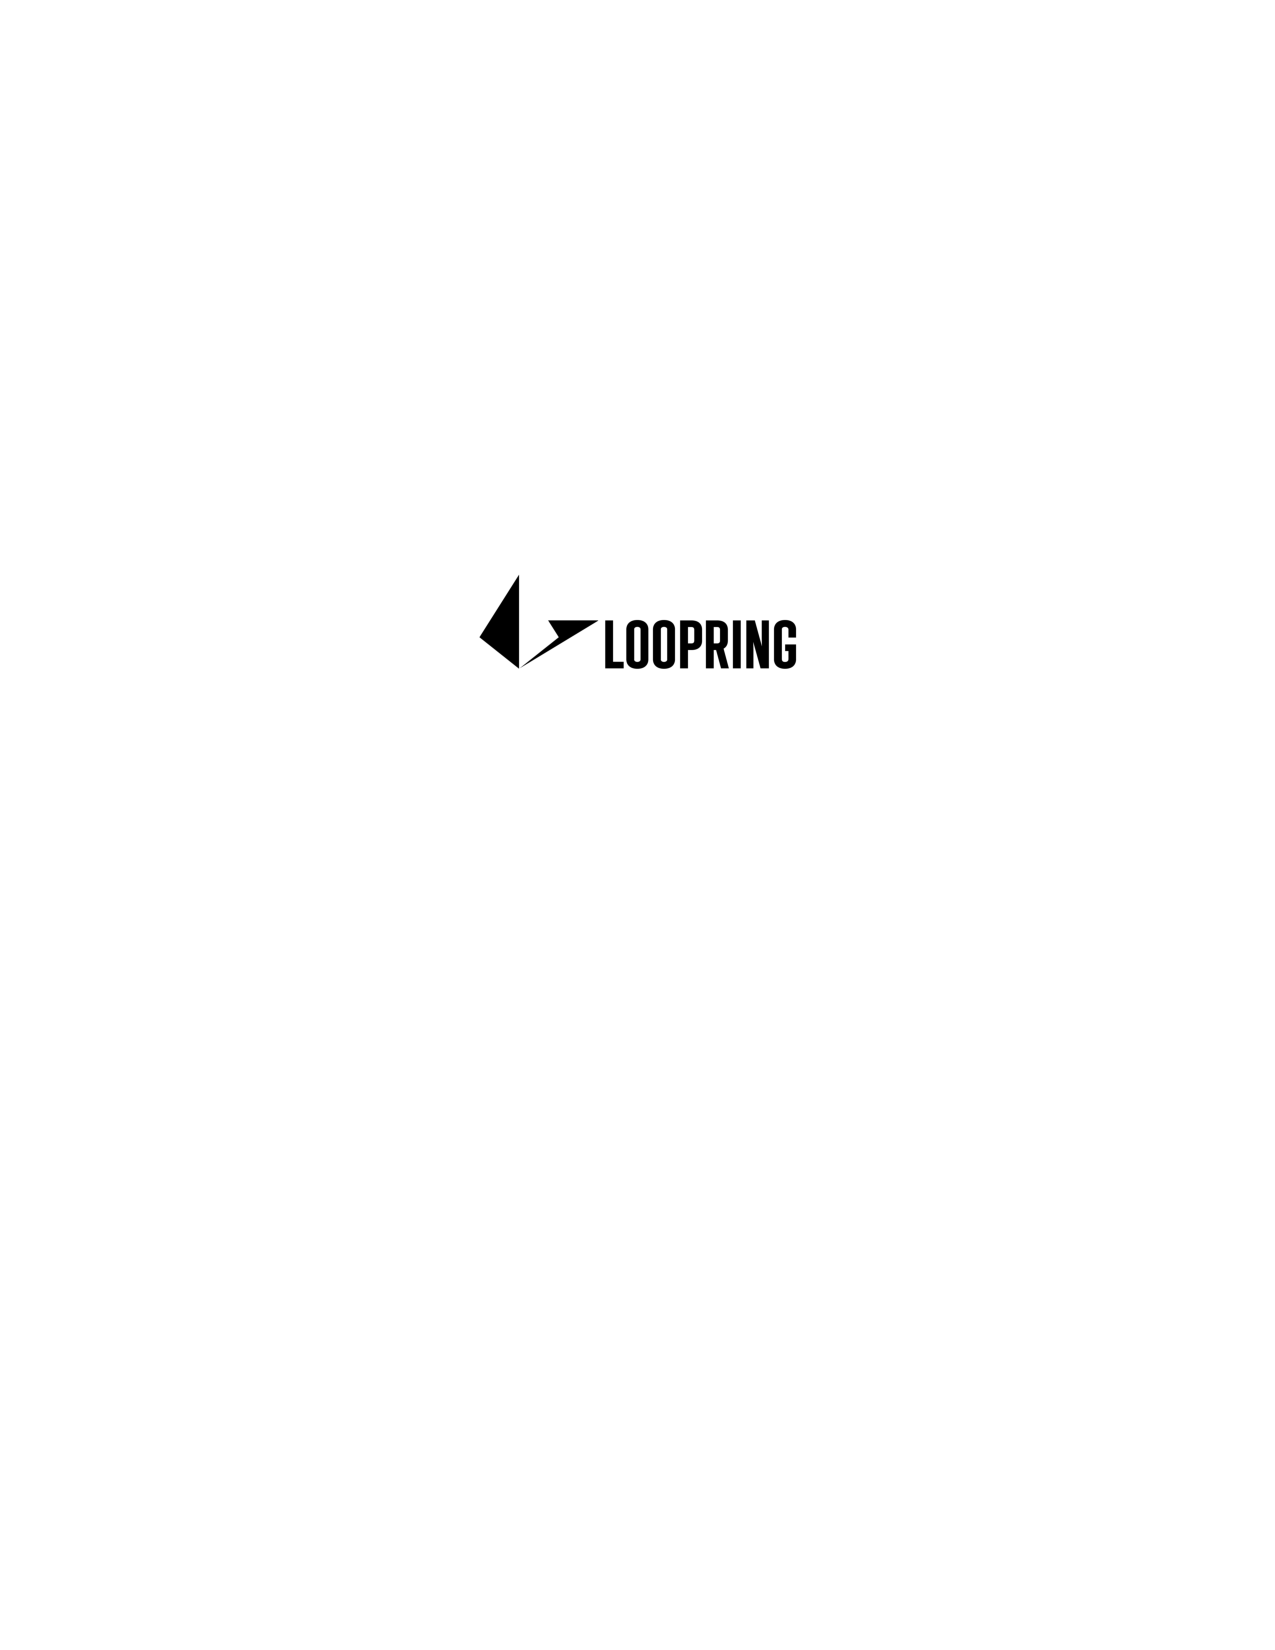
\includepdf[pages=1]{cover}
\hyphenpenalty=750

\title{\textbf{路印:}\\\textbf{去中心化代币交易协议}}
\author{
  王东\\
  \texttt{daniel@loopring.org}\\
  \and
  	周杰\\
  	\texttt{jay@loopring.org}\\
  	\and
  	王辉\\
  	\texttt{alex@loopring.org}\\
  	\and
  	Matthew Finestone\\
  	\texttt{matt.finestone@gmail.com}\\ 
  \\
  \texttt{https://loopring.org}
 }

\makeatletter
\def\CTEX@section@format{\Large\bfseries}
\makeatother

\makeatletter
\newenvironment{tablehere}
 {\def\@captype{table}}
 {}

\newenvironment{figurehere}
 {\def\@captype{figure}}
 {}
\makeatother
%
%\newcommand\BackgroundPic{%
%\put(0, 0){%
%\parbox[b][\paperheight]{\paperwidth}{%
%\vfill
%\centering
%\includegraphics[width=\paperwidth, height=\paperheight, %
%%keepaspectratio]{images/background.jpg}%
%]{images/background.jpg}%
%\vfill
%}}}


\begin{document}
%\AddToShipoutPicture{\BackgroundPic}
\maketitle


\begin{abstract}
路印是一项开放协议,用于构建去中心化交易所。它能充当公共智能合约,配合链下参与者撮合和广播订单,进行交易和结算。路印协议免费且可扩展, 为具备交易功能的去中心化应用(dApps)提供标准架构基石。路印协议使用互操作标准,实现零信任成本的匿名交易。与其他去中心化交易协议相比,路印在多笔撮合方面取得重大进展,消除交易代币种类的限制,极大提升流动性。针对不公平的抢先交易行为(在原始环路通过之前将交易写入区块),路印设计了一套独特而有效的防范方案。路印不依赖任何区块链系统,能够在任何区块链中部署智能合约功能。截止至撰文时,路印已成功在以太坊(Ethereum)\cite{buterin2017ethereum} \cite{wood2014ethereum} 和量子链(Qtum)\cite{dai2017smart} 上运行,在 NEO \cite{atterlonn2018distributed} 上开展部署。

\end{abstract}



\begin{multicols}{2}
\section{引言\label{sec:introduction}}

随着区块链资产激增,相应的交易需求亦同步上涨。与此同时,新种代币大量涌现,甚至连传统资产亦开始代币化,继而推动交易需求。无论交易代币的目的是出于投机,或是通过兑换原生实用代币接入代币所属网络;对于更广层面上的生态系统而言,加密资产之间的交易是其基本组成。事实上,资产是具有潜在能量 \cite{desotocapital}。若想解锁资本,释放其能量,需要确立资产所有权,区块链技术已给出一劳永逸的解决办法;还需要实现资产自由转移和转换。
 
因此,无需信任的代币(价值)交易便成为区块链技术用例中的焦点。然而,许多加密货币爱好者至今仍满足于在传统的中心化交易所中交易代币。正如比特币(Bitcoin) \cite{nakamoto2008bitcoin}所坚称,点对点电子现金\enquote{如果还依赖可信任第三方的介入,才可避免双重支付,就失去了原有优势。} 同理,去中心化资产如果必须借助可信赖的封闭中心化交易所进行交易,亦没有优势可言。可见市场对路印协议的迫切需求。

通过中心化交易所进行去中心化代币交易,从哲学上亦违背了去中心化项目所秉持的理念。另外,中心化交易所存在不少风险和限制,下文会对此进行详述。去中心化交易所(DEXs) \cite{schuh2015bitshares} \cite{bancor} \cite{kyber} 一直致力解决这些问题;亦确实有不少案例利用区块链作为交易中介,一定程度上缓解风险。一方面,DEXs 逐步成为新型经济的重要基础设施;另一方面,DEXs 运作性能亟待改善。路印的 dApp 不可知开放协议正是为构建上述基础设施提供模块化工具。

\section{交易所现状\label{sec:current_exchange_landscape}}

\subsection{中心化交易所的缺陷}
中心化交易所主要存在以下三种风险 1)低安全性;2)低透明度;3)低流动性

\textbf{低安全性} 源自用户一般将私钥(资金)交由中心化实体掌控。一旦中心化交易所遭受黑客恶意攻击,用户就有可能成为牺牲品。虽然,中心化交易所的安全隐患和入侵攻击 \cite{coincheckhack}  \cite{mcmillan2014inside}一直为人熟知,但大家一直视此为代币交易的 \enquote{赌注}。中心化交易所的服务器保管着上百万美元的用户资金,始终是黑客眼中的“肥肉”;交易所开发者在管理用户资金时亦偶有无心之失。简而言之,代币存入中心化交易所,便不受持有人控制。


\textbf{低透明度}让不正当交易所有机可乘,从而酿成风险。与上文的“低安全性”的区别在于,此处的风险由交易所运行者的不良动机引起。用户在使用中心化交易所时,交换的不是个人资产,而是借据(IOU)。当代币发送至交易所钱包,便交由交易所保管;交易所会用户提供相应的 IOU。此后的交易实际上都是用户之间的 IOU 交换。提取资产时,用户需向交易所交还 IOU,代币才可收管至交易所以外的用户钱包地址。整个过程缺乏透明度,交易所有可能突然关闭、冻结账户、破产等;亦有可能挪用所保管的资产,比如贷款给第三方。资产持有人即使不会因此损失一切,亦有可能承担高昂手续费、高峰期的交易延迟、监管风险和抢先交易等风险。

\textbf{低流动性}。从交易所运营者的角度出发,流动性断层会引起两种“赢者通吃”效应,打压新交易所进入市场。其一,拥有最多交易对的交易所会成为赢家,因为用户能够方便地在此完成全部交易。其二,拥有最深订单表的交易所亦会得益,因为每组交易代币都存在着有利价差。新交易所难以建立流动性,竞争力大受削弱。因此,即使用户怨声载道,甚至是发生严重黑客事件,许多中心化交易所依旧占有较高的市场份额。值得注意的是,随着中心化交易所市场占有率的提升,遭受入侵的风险亦同步上涨。


从用户角度出发,流动性断层对使用体验产生严重负面影响。在中心化交易所中,交易局限在平台的流动池、订单表及其所支持的交易对之中。资金持有人如果想将代币 \verb|A| 兑换成代币 \verb|B|, ,就必须选择同时支持两种代币的交易所;或是在不同的交易所中,以个人信息注册账户。通常情况下,持有人还需采取预备或中间交易,一般是兑换成比特币(BTC)或以太币(ETH),过程中需要支付价差。最后,有可能由于订单表深度不足,用户为了完成交易而被迫压缩订单。即使交易所宣称能够支持大宗交易,亦难以辨别所谓交易量和流动性的真伪 \cite{fakevolume}。

产物与传统金融系统相仿:流动性断层和生态系统相互隔离,造成大量交易集中在少数交易所中。区块链承诺的环球资金流动只会夭折在中心化交易所腹中。

\subsection{去中心化交易所的缺陷}
去中心化交易所与中心化交易所的部分区别在于,前者的交易直接在底层区块链上进行,用户得以控制自己的私钥(资产)。借助加密货币无需信任的技术,去中心化交易所规避了许多上文提到的安全风险,但在运行和架构限制方面仍存在缺陷。

流动性依旧是去中心化交易所时常面临的问题,用户需要在不同的流动池和和平台标准之间搜索交易对手。如果大多数 DEXs 或 dApps 标准不统一而无法实行互操作,订单不能在广阔的网络中分享或广播,就会出现流动断层效应。限价订单表流动性——准确而言,是回弹能力,即限价单成交后的更新速度,可能对用户的最优交易策略产生极大影响 \cite{limitorderliquidity}。缺乏统一标准不仅会制约流动性,还会让用户暴露于大量潜在安全隐患的专有智能合约。

再者,由于交易在链上进行,DEXs 继而受到底层区块链的限制,即规模化能力有限、执行(挖矿)延迟,以及更改订单的费用高昂。由于在区块链上执行代码需支付费用(油费),取消多份订单的代价高得吓人,导致基于区块链的订单表难以扩展。

最后,因为区块链订单表是公开的,矿工可以看到每笔交易。而订单在等待矿工写入新区块、添加到订单表的过程可能产生延迟,用户因此而面临抢先交易的风险,可能导致交易最终以不利价格或执行方式成交。

\subsection{综合解决方案}
基于上述原因,单纯依靠区块链的交易所局限诸多,难以与中心化交易所竞争。其实可取二者之长,将前者的免信任特质与后者的高速交易和灵活订单合二为一。路印和 0x \cite{warren20170x} 等协议发展出链上交易结合链下订单管理的解决方案。这些解决方案建立在开放智能合约之上;部分功能转移到链下,并赋予节点灵活性,使其在网络中扮演更重要的角色——双管齐下,突破去中心化交易所的规模化局限。即便如此,综合解决方案依然存在缺陷 \cite{costofdecent}。在本篇白皮书中,路印协议提出重大改进措施,完善综合解决方案。


\section{路印协议\label{sec:loopring_protocol}}
路印不是 DEX,而是模块化协议,帮助在不同区块链上构建 DEX。设计者拆解了传统交易所,用一套公共智能合约和去中心化参与者对其进行重组。路印网络由钱包、中继、流动性共享联盟链、订单表浏览器、环路矿工和资产代币化服务组成。在解释这些组成部分之前,必须先了解路印订单。

\subsection{订单环路\label{sec:order_ring}}
路印订单可表述为“单向订单模式(UDOM)”\cite{coinport2014udom}。UDOM 将订单表达为代币交易请求“卖出/买入数额(amountS/amountB)”,而非卖单和买单。此时,每笔订单实际上是两种代币之间汇率,路印协议从而获得一种强大功能,可以通过订单环路将多份订单混合和配对。有别于传统的一对一交易,路印的订单类型可高达 16 种,极大提高流动性和价格增长潜力。

\begin{center}
\begin{figurehere}
\centering
\tikzstyle{block} = [draw, fill=blue!20, rectangle, 
    minimum height=3em, minimum width=6em]
\tikzstyle{sum} = [draw, fill=blue!20, circle, node distance=1cm]
\tikzstyle{input} = [coordinate]
\tikzstyle{output} = [coordinate]
\tikzstyle{pinstyle} = [pin edge={to-,thin,black}]

\begin{tikzpicture}[
    auto, 
    node distance=2cm,
    >=latex',
    font=\bfseries\footnotesize\sffamily,
    order/.style={
		scale=0.7,
		rectangle,
		rounded corners,
		draw=black, 
		text centered,
%		text width=5cm,
		minimum height=12mm,
		fill=white
	},
	label/.style={
		scale=0.7
	}
  ]
    % We start by placing the blocks

  \node [order] (order2) 
 {%
 \begin{tabular}{l}
  \textbf{订单\#2}\\
  \textbf{持有人: Y}\\
  \textbf{卖出数额:9B}\\
  \textbf{买入数额: 12C}
 \end{tabular}
 };
 
  \node [order, below of=order2, xshift=-3.5cm] (order1) 
 {%
 \begin{tabular}{l}
  \textbf{订单\#1}\\
  \textbf{持有人:X}\\
  \textbf{卖出数额:10000A}\\
  \textbf{买入数额:2B}
 \end{tabular}
 };
 
 
  \node [order, below of=order2, xshift=3.5cm] (order3) 
 {%
 \begin{tabular}{l}
  \textbf{订单\#3}\\
  \textbf{持有人:Z}\\
  \textbf{卖出数额:100C}\\
  \textbf{买入数额:160A}
 \end{tabular}
 };
 
 \draw [draw,->] (order1) -- node [label] {\textbf{7898A}} (order3);
 \draw [draw,->] (order2) -| node [label, xshift=-1.8cm] {\textbf{8B}} (order1);
 \draw [draw,->] (order3) |- node [label, xshift=1cm, yshift=0.24cm] {\textbf{98C}} (order2);

\end{tikzpicture}

\caption{由 3 笔订单组成的订单环路}
\label{fig:ring}
\end{figurehere}
\end{center}


上图所示的订单环路由 3 笔订单组成。每笔订单计划卖出的代币(\verb|tokenS|)恰好是另一笔订单计划买入的代币(\verb|tokenB|),由此形成的环路使得每笔订单都能获得想要的代币,而不必直接与交易对相应的订单交易。传统的订单配对交易依然成立,其实本质上是订单环路的特例。 

\begin{definition}[订单环路] 设 $C_{0}$, $C_{1}$, $\cdots$, $C_{n-1}$ 为 $n$ 种代币, $O_{0\rightarrow 1}$, $\cdots$, $O_{i\rightarrow i\oplus 1}$, $\cdots$, $O_{n-1 \rightarrow 0}$ 为 n 笔订单。这些订单可组成交易订单环路:
$$O_{0\rightarrow 1} \rightarrow \cdots \rightarrow O_{i\rightarrow i\oplus 1} \rightarrow \cdots \rightarrow O_{n-1\rightarrow 0} \text{, }$$
其中 $n$ 为订单环路的长度,且 $i\oplus 1 \equiv i+1 \mod n$。
\end{definition}

当所有组成交易的执行汇率等同或优于用户的暗中出价,订单环路即可成立。为了验证订单环路是否有效,路印协议智能合约必须确认环路矿工提交的订单环路中,所有订单的原始汇率乘积大于等于1。

假设 Alice 和 Bob 想要交易代币 \verb|A| 和代币 \verb|B|。Alice 希望以 15 个代币 \verb|A| 换取 4 个代币 \verb|B| ;Bob 希望以 10 个代币 \verb|B| 换取 30 个代币 \verb|A| 。

在此,谁是买方,谁是卖方呢?取决于用哪种代币作为价格参考。如果以代币 \verb|A| 为参考,Alice 购买代币 \verb|B| 的期望汇率是 ${15 \over 4} = 3.75$\verb|A|,而 Bob 则以 ${30 \over 10} = 3.00$\verb|A|的汇率出售 10 个代币 \verb|B|。如果以代币 \verb|B|为参考,Alice 出售 15 个代币 \verb|A| 的汇率是 ${4\over 15}=0.26666667$\verb|B|,而 Bob 则期望以 ${10 \over 30}=0.33333334$\verb|B|的汇率买入 10 个代币 \verb|A|。因此,并不存在绝对的买卖方。

在第一种情况中,Alice 愿意支付的价格 ($3.75$\verb|A|) 高于 Bob 开出的售价  ($3.00$\verb|A|),而第二种情况下,Bob 愿意支付的价格 ($0.33333334$\verb|B|) 高于 Alice 开出的售价 ($0.26666667$\verb|B|)。显然,买方出价大于或等于卖方出价时,交易即可达成。

\begin{equation}
{{15\over 4} \over {30\over 10}} = {{10\over 30} \over {4\over 15}}={15 \over 4} \cdot {10 \over 30} = 1.25 > 1
\end{equation}

因此,为确认一组由 $n$ 笔订单组成的集合是否能够部分或完全成交,必须知道每笔订单的汇率乘积是否大于或等于 1。是的话,这 $n$ 笔订单就可以部分或全部成交 \cite{supersymmetry}。

倘若引入第三方 Charlie。此时,Alice 想以 $x_1$ 个代币 \verb|A| 换取 $y_1$ 个代币 \verb|B|,Bob 想以 $x_2$ 个代币 \verb|B| 换取 $y_2$ 个代币 \verb|C|, ,Charlie 想以 $x_3$ 个代币 \verb|C| 换取 $y_3$ 个代币 \verb|A|。代币种类已经齐全,只要满足以下条件,交易即可能达成:

\begin{equation}
{{x_1 \cdot x_2 \cdot x_3 \over y_1 \cdot y_2 \cdot y_3} \geq 1}
\end{equation}


更多关于路印订单的细节见章节 \ref{anatomy}。



\section{生态系统参与者\label{sec:ecosystem}}
有赖以下参与者的协作,路印生态系统能够涵盖中心化交易所的所有功能。

\begin{itemize}

\item \textbf{钱包}:一种常见的钱包服务或界面,用户可由此使用代币,亦可向路印网络发送订单。钱包与环路矿工分享手续费,从而激励订单生成(见章节 \ref{sec:token})。为了推动未来的交易转移至用户个人钱包的安全范围内进行,关键的一步是通过路印协议连接资金流动池。

\item \textbf{流动性共享联盟链/中继网}: 一种用于订单和流动性共享的中继网。节点在运行路印中继软件时,可以通过联盟链加入现成网络,与其他中继共享流动性。我们正在构建的首条联盟链达到接近实时的订单共享(1-2 秒出块时间),同时调整过往记录,加快新节点的下载速度。需要指出的是,路印协议不强求中继加入联盟链。中继可选择独立运行,不和其他中继共享流动性;或是创建及管理属下的流动性共享网络。

\item \textbf{中继/环路撮合}:中继作为节点,从钱包或中继网络接收订单,维护公共订单表和交易历史,同时(通过任意环路中介)有选择地向其他中继或中继网络节点广播订单。交易撮合是中继的功能,但不是必然属性;运行过程需要庞大计算力,全盘在链下进行。能够进行交易撮合的中继称为\enquote{环路矿工(Ring-Miners)},通过配对多笔订单搭建交易环路。中继可以自由选取(1)与其他中继的沟通方式;(2)构建订单表的方式,以及(3)撮合交易环路的方式(挖矿算法)。


\item \textbf{路印协议智能合约(LPSC)}:一套免费的公共智能合约,检验环路矿工发出的订单环路,为用户在结算及代币转账过程中免除第三方信任,以手续费激励环路矿工和钱包,以及发布事务。中继/订单浏览器监听这些事务,相应地更新订单表和交易历史。详见附录 \ref{app:protocol_ethereum}。

\item \textbf{资产代币化服务(ATS)}:此项中心化服务由可靠的公司和机构负责,桥接无法直接在路印协议上交易的资产。用户寄存实物、法币或其他链上代币等资产,以此获得的代币可在未来赎回资产。虽然路印目前仍然不是跨链交易协议(有待合适解决方案),但 ATS 可实现 ERC20 代币 \cite{ERC20} 与实物资产、其他区块链资产之间的交易。 

\end{itemize}


\section{交易流程\label{sec:process}}



\begin{enumerate} 


\item \textbf{协议授权}:如图 \ref{fig:process} 所示,用户 \verb|Y| 想交易代币,因此授权 LPSC 出售数额为 \verb|amountS| 的代币 \verb|B|。此操作不会冻结用户的代币;订单处理期间,用户依然可以自由支配代币。

\item \textbf{订单创建}: 订单浏览器等中继和其他网络中介提供代币 \verb|B| 和代币 \verb|C|之间的当前汇率和订单表。用户 \verb|Y| 通过任意综合钱包界面发出订单(限价订单),确定卖出数额 \verb|amountS| 和买入数额 \verb|amountB| 等参数。订单可附带一定数额的 LRx,作为支付环路矿工的手续费。LRx 数额越高,订单便更有可能及早得到环路矿工的处理。订单的哈希值以用户 \verb|Y|的私钥签署。

\item \textbf{订单广播}:钱包向单个或多个中继发送订单及其签名,中继随之更新辖下公共订单表。路印协议不限制订单表架构,允许“先到先得”模式;中继可以自行选择订单表设计。

\item \textbf{流动性共享}:中继可通过任意沟通媒介,向其他中继广播订单。在此再次强调,节点有权选择是否及如何交流。为了保证网络具有稳定流通能力,联盟链内置了流动性共享中继网络。正如上文所述,该中继网络有利于提高速度和包容性。

\begin{center}
\begin{figurehere}
\centering
\tikzstyle{block} = [draw, fill=blue!20, rectangle, 
    minimum height=3em, minimum width=6em]
\tikzstyle{sum} = [draw, fill=blue!20, circle, node distance=1cm]
\tikzstyle{input} = [coordinate]
\tikzstyle{output} = [coordinate]
\tikzstyle{pinstyle} = [pin edge={to-,thin,black}]

\begin{tikzpicture}[
    auto, 
    scale=0.7,
    node distance=2cm,
    >=latex',
    font=\bfseries\footnotesize\sffamily,
    order/.style={
		rectangle,
		scale=0.7,
		rounded corners,
		draw=black, 
		text centered,
%		text width=5cm,
		minimum height=12mm,
		minimum width=30mm,
		fill=white
	},
	role/.style={
		circle,
		scale=0.7,
		draw=black, 
		text centered,
%		text width=5cm,
		minimum height=12mm,
		minimum width=12mm,
		fill=white
	},
	steps/.style={
		circle,
		scale=0.7,
		draw=black, 
		text centered,
%		text width=5cm,
%		minimum height=12mm,
%		minimum width=12mm,
		fill=black,
		text=white
	},
	account/.style={
		circle,
		scale=0.7,
		draw=black, 
		text centered,
%		text width=5cm,
		minimum height=16mm,
		minimum width=16mm,
		fill=white
	},
	label/.style={
	  scale=0.7
    }
  ]

 
 \node [role] (user1)  {用户 X};
 \node [role, below of=user1] (user2)  {用户 Y};
 \node [role, below of=user2] (user3)  {用户 Z};
 \node [role, below of=user3, fill=gray!20] (relay1)  {中继 M};
 \node [role, below of=relay1, fill=gray!20] (relay2)  {中继 N};

 
 \node [order, left of=user1, xshift=-1cm] (order1) 
 {%
 \begin{tabular}{l}
  \textbf{订单 1}\\
  \textbf{持有人:X}\\
  \textbf{卖出数额:10000 A}\\
  \textbf{买入数额:2 B}
 \end{tabular}
 };
 
 \draw [draw, ->]  (user1) -- (order1) [label]{};
 \draw [bend right,->] (order1) to node [auto, scale=0.7] {} (relay1);
 \draw [bend right,->] (order1) to node [auto, scale=0.7] {} (relay2);
% \draw [draw, ->]  (order1) |- (relay1) [label]{};
% \draw [draw, ->]  (order1) |- (relay2) [label]{};
 
 \node [order,left of=user2, xshift=-1.5cm] (order2) 
 {%
 \begin{tabular}{l}
  \textbf{订单 2}\\
  \textbf{持有人:Y}\\
  \textbf{卖出数额:9  B}\\
  \textbf{买入数额:12 C}
 \end{tabular}
 };
 \draw [draw, ->]  (user2) -- (order2) [label]{};
 \draw [bend right,->] (order2) to node [auto, scale=0.7] {} (relay1);
 \draw [bend right,->] (order2) to node [auto, scale=0.7] {} (relay2);
% \draw [draw, ->]  (order2) |- (relay1) [label]{};
% \draw [draw, ->]  (order2) |- (relay2) [label]{};
% 
\node [order, left of=user3, xshift=-2cm] (order3) 
 {%
 \begin{tabular}{l}
  \textbf{订单 3}\\
  \textbf{持有人:Z}\\
  \textbf{卖出数额:100 C}\\
  \textbf{买入数额:160 A}
 \end{tabular}
 };
 \draw [draw, ->]  (user3) -- (order3) [label]{};
 \draw [bend right,->] (order3) to node [auto, scale=0.7] {} (relay1);
 \draw [bend right,->] (order3) to node [auto, scale=0.7] {} (relay2);
% \draw [draw, ->]  (order3) |- (relay1) [label]{};
% \draw [draw, ->]  (order3) |- (relay2) [label]{};
 
% // The Ring
\node [order, 
yshift=-1.5cm,
xshift=-2.75cm,
below of=relay2,
fill=gray!10,
minimum width=4.2cm,
minimum height=5cm] (ring) {};


\node [order, dashed, below of=relay2,yshift=-0.2cm,xshift=-2.5cm] (order11) 
 {%
 \begin{tabular}{l}
  \textbf{订单 1}\\
  \textbf{持有人:X}\\
  \textbf{卖出数额:10000 A}\\
  \textbf{买入数额:2 B}
 \end{tabular}
 };
 \node [order, dashed,below of=order11,xshift=-0.25cm,yshift=0.7cm] (order21) 
 {%
 \begin{tabular}{l}
  \textbf{订单 2}\\
  \textbf{持有人:Y}\\
  \textbf{卖出数额:9  B}\\
  \textbf{买入数额:12 C}
 \end{tabular}
 };
\node [order, dashed,below of=order21,xshift=-0.25cm,yshift=0.7cm] (order31) 
 {%
 \begin{tabular}{l}
  \textbf{订单 3}\\
  \textbf{持有人:Z}\\
  \textbf{卖出数额:100 C}\\
  \textbf{买入数额:160 A}
 \end{tabular}
 };
 
 % // The blockchain
\node [
rectangle,
fill=gray!20, 
right of=user1,
yshift=-4.5cm,
xshift=0.1cm,
scale=0.7,
minimum width=3.2cm,
minimum height=15.6cm] (blockchain) {\parbox[b][15cm]{1.3cm}{区块链}};
% blockchain accounts
  \node [account, right of=user1, xshift=1cm] (account1)  {账户X};
  \node [account, right of=user2, xshift=1cm] (account2)  {账户Y};
  \node [account, right of=user3, xshift=1cm] (account3)  {账户Z};
  \node [account, right of=relay1, xshift=1cm] (account4)  {账户M};
  \node [account, right of=relay2, xshift=1cm] (account5)  {账户N};
  \node [account, double, below of=account5, yshift=-1.5cm] (psc)  {LPSC};
  
 \draw [draw, ->]  (user1) -- (account1) [label]{};
 \draw [draw, ->]  (user2) -- (account2) [label]{};
 \draw [draw, ->]  (user3) -- (account3) [label]{};
% \draw [draw, ->]  (relay1) -- (account4) [label]{};
% \draw [draw, ->]  (relay2) -- (account5) [label]{};
 \draw [draw, double, thick]  (relay1) to node [auto, scale=0.7] {共享流动性}  (relay2) [label]{};
% \draw [draw, ->]  (relay1) -- (ring) [label]{};
 \draw [draw, ->]  (relay2) to node [auto, scale=0.7, xshift=-1.8cm, yshift=0.3cm] {环路撮合}  (ring) [label]{};
 \draw [draw, ->]  (ring) to node [auto, scale=0.7] {提交环路} (psc) [label]{};
 
 \draw [bend left,->] (account1) to node [auto, scale=0.7] {\textbf{7898 A}} (account3);
 \draw [bend left,->] (account2) to node [auto, scale=0.7] {\textbf{8 B}} (account1);
 \draw [bend left,->] (account3) to node [auto, scale=0.7] {\textbf{98 C}} (account2);
 
 \draw [bend left,->, dashed] (account1) to node [auto, scale=0.7] {} (account5);
 \draw [bend left,->, dashed] (account2) to node [auto, scale=0.7] {} (account5);
 \draw [bend left,->, dashed] (account3) to node [auto, scale=0.7, xshift=.5cm] {\textbf{手续费}} (account5);
  
  
% \draw [draw,->] (order1) -- node [label] {\textbf{7898 A}} (order3);
% \draw [draw,->] (order2) -| node [label, xshift=-1.8cm] {\textbf{8 B}} (order1);
% \draw [draw,->] (order3) |- node [label, xshift=1cm, yshift=0.24cm] {\textbf{98 C}} (order2);

\node [steps, right of=user2, xshift=-0.6cm] () {1};
\node [steps, left of=user2, xshift=0.8cm] () {2};
\node [steps, left of=relay2, xshift=0.3cm, yshift=1cm] () {3};
\node [steps, left of=relay1, xshift=3.3cm, yshift=-1.6cm] () {4};
\node [steps, below of=relay2, xshift=-0.2cm, yshift=0.4cm] () {5};
\node [steps, right of=account3, xshift=-0.6cm] (step5) {6};

 \draw [bend right, ->]  (psc) to node [auto, scale=0.7, xshift=0.5cm] {结算} (step5) [label]{};
 
\end{tikzpicture}

\caption{路印交易流程}
\label{fig:process}
\end{figurehere}
\end{center}



\item \textbf{环路撮合(订单配对)}:环路矿工撮合多笔订单,以等同或优于用户开出的汇率满足部分或全部订单数额。路印协议之所以能够保证任何交易对之间的高流动性,很大程度上得益于环路矿工。如果成交汇率高于用户 Y 的出价,环路中所有订单皆可共享个中利润。而作为报酬,环路矿工可以选择收取部分利润(分润,同时向用户支付 LRx),或收取原定的 LRx 手续费。

\item \textbf{验证及结算}:LPSC 接收订单环路后会进行多项检查,验证环路矿工提供的数据,决定订单环路是否可以部分或全部结清(取决于环路订单的成交汇率和用户钱包中的代币余额)。如果各项检查达标,合约会通过原子操作将代币转至用户,同时向环路矿工和钱包支付手续费。LPSC 如果发现用户 \verb|Y|的余额不足,会采取缩减订单数额;一旦足够的资金存入地址,订单会自动恢复至原始数额。而取消订单则需要单向手动操作且不可撤销。


\end{enumerate}





%
%\end{multicols}
%
%\begin{center}
%\begin{figurehere}
%\includegraphics[height=8cm]{images/en_protocol.png}
%\caption{Loopring Trading Process}
%\label{fig: Loopringrotocol}
%\end{figurehere}
%\end{center}
%
%\begin{multicols}{2}

\section{操作灵活性\label{sec:business_model}}
值得注意的是,在路印开放标准下,参与者享有灵活的操作空间,可自由采取新型商业模式,为用户提供价值,从中根据交易量或其他度量赚取相应 LRx 手续费。生态系统由多模块组成,旨在从多方应用支持参与者。


\subsection{订单表\label{sec:order_book}}
中继在设计订单表时,可选择各种方式展示和配对用户订单。路印实行的首个订单表遵从 OTC 模式,限价订单仅根据价格排序。换而言之,订单表排列忽略订单的时间戳。然而,中继亦可仿效典型中心化交易所配对引擎,将订单表设置成根据价格排列订单,同时考虑到时间戳顺序。如果中继倾向于此类订单表,可以选择配置钱包;由钱包将订单单独发送至某个中继,再由改中继根据时间顺序撮合订单。总之,任何类似的架构都可行。


尽管其他 DEX 协议有可能要求中继持有一定资源——起始代币余额以接收订单;而路印中继只需找到配对订单即可达成交易,因此无须储备起始代币。

\subsection{流动性共享\label{sec:liquidity_sharing}}
中继可自行选择共享流动性(订单)的方式。路印联盟链只是共享方案之一;路印生态系统下,中继可随意沟通交流。除了加入联盟链以外,中继还可创建和管理辖下的流动性共享网络,订立合适的规则和激励机制。中继亦可独立运行,比如上文提到的示例方案中,中继可利用钱包实现订单的按时顺序。当然,在提高网络效率方面,与其他中继沟通得到的好处是显而易见;然而,不同商业模式需要特定的流动性分享和手续费分摊机制。


\section{Protocol 协议细节\label{sec:protocol}}

\subsection{剖析订单\label{anatomy}}
订单是一组数据,描述用户交易意向。路印订单的定义遵从“单向订单模式(UDOM)”,具体如下:

\begin{verbatim}
  message Order {
    address protocol;
    address owner;
    address tokenS;
    address tokenB;
    uint256 amountS;
    uint256 amountB;
    unit256 lrcFee
    unit256 validSince; // Seconds since epoch
    unit256 validUntil; // Seconds since epoch
    uint8   marginSplitPercentage;  // [1-100]
    bool    buyNoMoreThanAmountB;
    uint256 walletId;
    // Dual-Authoring address(双重授权地址)
    address authAddr;
   	// v, r, s are parts of the signature( v, r, s 是签名组成部分)
    uint8   v;       
    bytes32 r;
    bytes32 s;
    // Dual-Authoring private-key,(双重授权私钥)
    // not used for calculating order's hash,(不用作订单哈希值计算)
    // thus it is NOT signed.(因此不签署)
    string  authKey;          
    uint256 nonce;
  }
\end{verbatim}


为了证明来源,订单以用户私钥签署 \verb|authAddr|除外的参数哈希值; \verb|authAddr| 参数则用作签署订单所属的环路,防范抢先交易,详见章节 \ref{sec:dual_authoring} 。订单签名以 \verb|v|、\verb|r|和 \verb|s| 字段表示,与订单参数一同发送至网络。此举保证订单在整个生命周期中无法变更。即便如此,协议仍可根据地址余额和其他变量计算出订单当前状态。



UDOM 不包含固定价钱(本质上必须是浮点数),而是使用术语“汇率( \verb|rate|)或“$r$” ,表达成“卖出数额/买入数额(\verb|amountS|/\verb|amountB|)”。汇率不是浮点数,而是表达式;仅在有需要的情况下使用其他无符号整数计算,将所用中间结果算作无符号整数,从而提高计算精度。

\subsubsection{买入数额}

环路矿工撮合订单时,可能会找到优于用户出价的汇率,用户最终获得的代币数额高于订单设定的买入数额。然而,如果启动 \verb|buyNoMoreThanAmountB| 指令(设定为 \verb|True|), 协议则会确保用户所得代币数额不超过订单设定的买入数额。因此,UDOM 的 \verb|buyNoMoreThantokenB|指令决定订单何时完全达成。与传统买/卖单相比,\verb|buyNoMoreThantokenB| 为卖出或买入数额设置上限,允许用户更细致地表达交易意向。

例如,设卖出数额 \verb|amountS| = 10, 买入数额 \verb|amountB| = 2,汇率 $r$ = 10/2 = 5。此时,用户愿意以 5 个代币 \verb|tokenS| 换取 1 个代币 \verb|tokenB|;环路矿工找到汇率为 4 的订单,意味着用户可以获得 2.5 个代币 \verb|tokenB| ,高出预期的 2 个。然而,如果用户只想要 2 个代币 \verb|tokenB|,将交易设定为 \verb|buyNoMoreThanAmountB|,LPSC performs便会以汇率 4 成交订单,以 4 个代币 \verb|tokenS| 换成每个代币 \verb|tokenB|,从而节省 2 个代币 \verb|tokenS|;计算尚未考虑撮合手续费(见章节 \ref{sec:fee_model})。

诚然,如果我们用以下形式


\begin{verbatim}
	      Order(amountS,tokenS,
	            amountB,tokenB,
	            buyNoMoreThantokenB)
\end{verbatim}

简单地表达订单;在传统交易所中的 ETH/USD 市场,传统买卖模式可表达以下第 1 种和第 3 种订单,但无法表达其余两种订单:

\begin{enumerate}
	\item 以 300 USD/ETH 的价格卖出 10 个 ETH;订单可表达为:\verb|Order(10, ETH, 3000, USD, False)|。
	\item 以 300 USD/ETH 的价格出售 ETH,换取 3000 USD;订单可表达为:\verb|Order(10, ETH, 3000, USD, True)|。
	\item 以 300 USD/ETH 的价格买入 10 个 ETH;订单可表达为:\verb|Order(3000, USD, 10, ETH, True)|。
	\item Spend以 300 USD/ETH 的价格和 3000 USD 换取尽量多的 ETH;订单可表达为:\verb|Order(3000, USD, 10, ETH, False)|。
\end{enumerate}



\subsection{环路验证\label{sec:ring_verification}}

LPSC 不进行交易汇率或数额计算,而负责接收和验证环路矿工提交的数值。计算交由环路矿工完成主要出于两个原因:(1)以太坊的 solidity\cite{dannen2017introducing} 等智能合约编程语言不支持浮点数,尤其是工作量证明 $pow(x, 1/n)$(计算⼀个浮点数的 n 次⽅根);(2)计算转移到链下进行,可以降低区块链计算负担和成本。


\subsubsection{子环路验证\label{sec:sub_ring_check}}
这步程序防止套利者在已有订单环中加入新订单,不正当地牟取利润。环路矿工找到有效订单环路后,有可能受到利益驱使,额外加入新的订单,从而获取用户的全部利润(汇率折价)。如下图 \ref{fig:subring} 所示,仔细计算 $x1$, $y1$, $x2$ 和 $y2$,即可使环路中所有订单汇率的乘积刚好等于 1,从而避免汇率折价。

\begin{center}
\begin{figurehere}
\centering
\tikzstyle{block} = [draw, fill=blue!20, rectangle, 
    minimum height=3em, minimum width=6em]
\tikzstyle{sum} = [draw, fill=blue!20, circle, node distance=1cm]
\tikzstyle{input} = [coordinate]
\tikzstyle{output} = [coordinate]
\tikzstyle{pinstyle} = [pin edge={to-,thin,black}]

\begin{tikzpicture}[
    auto, 
    node distance=2cm,
    >=latex',
    font=\bfseries\footnotesize\sffamily,
    order/.style={
		scale=0.7,
		rectangle,
		rounded corners,
		draw=black, 
		text centered,
%		text width=5cm,
		minimum height=12mm,
		fill=white
	},
	label/.style={
		scale=0.7
	}
  ]
    % We start by placing the blocks

  \node [order] (order2) 
 {%
 \begin{tabular}{l}
  \textbf{订单 2}\\
  \textbf{持有人:Y}\\
  \textbf{卖出数额:9B}\\
  \textbf{买入数额:12C}
 \end{tabular}
 };
 
  \node [order, below of=order2, xshift=-3.5cm] (order1) 
 {%
 \begin{tabular}{l}
  \textbf{订单 1}\\
  \textbf{持有人:X}\\
  \textbf{卖出数额:10000 A}\\
  \textbf{买入数额:2 B}
 \end{tabular}
 };
 
 
  \node [order, below of=order2, xshift=3.5cm] (order3) 
 {%
 \begin{tabular}{l}
  \textbf{订单 3}\\
  \textbf{持有人:Z}\\
  \textbf{卖出数额:100 C}\\
  \textbf{买入数额:160 A}
 \end{tabular}
 };
 
   \node [order, below of=order3, fill=gray!20] (order4) 
 {%
 \begin{tabular}{l}
  \textbf{订单 4}\\
  \textbf{持有人:M}\\
  \textbf{卖出数额: x1 A}\\
  \textbf{买入数额:y1 B}
 \end{tabular}
 };
 
 
  \node [order, below of=order1, fill=gray!20] (order5) 
 {%
 \begin{tabular}{l}
  \textbf{订单 5}\\
  \textbf{持有人:addressM}\\
  \textbf{卖出数额:x2 C}\\
  \textbf{买入数额:y2 A}
 \end{tabular}
 };
 
 \draw [draw,->] (order1) -- node [label, xshift=-2cm] {} (order5);
 \draw [draw,->] (order2) -| node [label, xshift=-1.6cm] {} (order1);
 \draw [draw,->] (order3) |- node [label, xshift=1cm] {} (order2);
 \draw [draw,->] (order4) -- node [label, xshift=1.8cm] {} (order3);
 \draw [draw,->] (order5) -- node [label, yshift=0.2cm] {} (order4);
  
\end{tikzpicture}

\caption{带有子环路的订单环路}
\label{fig:subring}
\end{figurehere}
\end{center}

矿工这种做法虽然对网络不构成任何风险,但亦不会增加任何价值,路印视此为不公正行为。为了预防这种情况发生,路印协议规定有效的订单环路不能够含有任何子环路。LPSC 会确保同一个代币不能两次买入或卖出。从上图可见,代币 \verb|A|两次用作卖出和买入,这是路印所不允许的。


\subsubsection{成交汇率验证\label{sec:fill_rate_check}}


订单环路的汇率由环路矿工负责计算,原因已在上文阐述;LPSC 则负责验证计算是否准确。首先,LPSC 检查矿工为每张订单执行的汇率小于或等于用户设定的买入汇率,确保用户以等同或高于期望值的汇率完成交易。汇率验证通过后,LPSC 会进一步确认环路中每笔订单的汇率折价是否相同。假设折价为 $\gamma$,每笔订单的价格则为:

$r_{0\rightarrow 1} \cdot (1-\gamma)$, $r_{1\rightarrow 2} \cdot (1-\gamma)$, $r_{2 \rightarrow 0} \cdot (1-\gamma)$, 且满足:
\begin{equation}
r_{0\rightarrow 1} \cdot (1-\gamma)\cdot r_{1\rightarrow 2} \cdot (1-\gamma) \cdot r_{2 \rightarrow 0} \cdot (1-\gamma) = 1
\end{equation}
得出: 
\begin{equation}
\gamma = 1- \frac{1}{\sqrt[3]{r_{0\rightarrow 1} \cdot r_{1\rightarrow 2} \cdot r_{2\rightarrow 0}}}\text{.}
\end{equation}
如果交易在 $n$ 笔订单之间进行,\texttt{折价} 则为:
\begin{equation}
\gamma = 1- \frac{1}{\sqrt[n]{\prod_{i=0}^{n-1} r^i}} \text{,}
\end{equation}

 $r^i$ 是第 $i$ 笔订单的周转率。显然,只有在折价 $\gamma \ge 0$ 时,这些订单才能达成;第 $i$ 订单($O^i$)的实际交易汇率为 $\hat{r^i} = r^i \cdot (1-\gamma)$, $\hat{r^i}\le r^i$。

借用上文给出的例子,Alice 想以 15 个代币 \verb|A| 换取 4 个代币 \verb|B|,Bob 想以 10 个代币 \verb|B| 换取 30 个代币 \verb|A| 。如果以代币 \verb|A| 为参考,Alice 买入代币 \verb|B| 的预期汇率是 $\frac{15}{4}$ = 3.75\verb|A|,而 Bob 出售代币 \verb|B| 的预期汇率是 $\frac{30}{10}$ = 3.00\verb|A|,折价计算则为 $\frac{150}{120}$ = 1.25 即 $\frac{1}{1.25}$ = 0.8 = $(1 −- \gamma)^2$。因此,对于双方都公平的汇率是以 $\sqrt{0.8}$ $\cdot$ 3.75 $\approx$ 3.3541 个代币 \verb|A| 换取每个代币 \verb|B|。

Bob 卖出 4 个代币 \verb|B|,获得 13.4164 个代币 \verb|A|,比预期的 12 要高。而 Alice 获得 4 个代币 \verb|B|,仅支付了 13.4164 个代币 \verb|A| 比预期的 15 要低。请注意,部分利润会用作手续费,奖励矿工(和钱包)。(见章节  \ref{sec:fee_model})。


\subsubsection{成交跟踪和取消}

用户如需取消部分或全部订单,可向 LPSC 发送特殊交易,当中包含订单细节和取消数额。LPSC 收到相关信息后,会将需要取消的数额记录在案,并向网络发布一项“订单取消( \verb|OrderCancelled|)”事务。此后,LPSC 追踪成交和取消的数额,并利用用户的哈希值作为标记储存数额。数据对外公开;数据出现变动时,“订单取消/订单成交(\verb|OrderCancelled| / \verb|OrderFilled|)”事务会同时发生。在订单环结算环节中,LPSC 跟踪数据这一步骤非常关键。

LPSC 可使用“订单取消( \verb|OrdersCancelled|)”事务取消某一地址下任意交易对的所有订单,或是“所有订单取消( \verb|AllOrdersCancelled|)”事务取消某一地址下的所有订单。


\subsubsection{按比例缩减订单\label{sec:order_scaling}}
根据成交和取消数额纪录,以及发送者账户的当前余额,订单会得到相应比例的缩减。系统筛选出成交数额最小的订单,以此为依据压缩环路中所有交易。


找出交易数额最低的订单,有助于计算出环路中每笔订单的成交数额。比如,第 $i$笔订单的交易数额为环路中最低,每笔订单卖出的代币数目 $\hat{s}$ 和每笔订单买入的代币数目 $\hat{b}$ 可通过如下方式计算:

\[
\begin{split}
&\hat{s}^{i}=\overline{s}_i\text{, } \hat{b}^{i}=\hat{s}^{i}/ \hat{r}^i\text{, }\text{;}\\
&\hat{s}^{i\oplus 1}=\hat{b}^i\text{, } \hat{b}^{i\oplus 1}=\hat{s}^{i\oplus 1}/ \hat{r}^{i\oplus 1}\text{;}\\
&\hat{s}^{i\oplus 2}=\hat{b}^{i\oplus 1}\text{, } \hat{b}^{i\oplus 2}=\hat{s}^{i\oplus 2}/ \hat{r}^{i\oplus 2}\text{;}\\
& ...
%\text{.}
\end{split}
\]
$\overline{s}_i$ 为订单部分成交后的余额。

实践过程中,我们可以认定环路的每笔订单持有最低数额,然后计算环路中每笔订单的成交数额,计算次数最多为两次。

例如,如果最低成交数额是原始订单的 5\%,环路中所有交易都会压缩至 5\%。交易达成后,之前作为最低数额参考的那笔订单实际上是全部成交。


\subsection{环路结算\label{sec:settlement}}

如果订单环路完成上述所有验证,环路即可封闭并达成交易。此时, $n$笔订单会相互连接成封闭订单环路,如图 4 所示:

\begin{center}
\begin{figurehere}
\centering
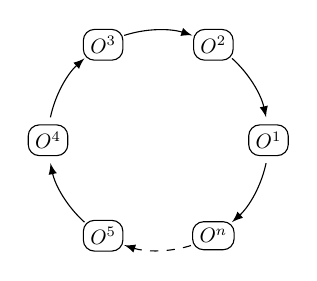
\begin{tikzpicture}[
circle/.style={
		scale=0.75,
		rounded corners,
		draw=black, 
		text centered,
		}
]

\def \n {6}
\def \m {4}
\def \radius {1.4cm}
\def \margin {12} % margin in angles, depends on the radius

\foreach \s in {1,...,\m}
{
  \node[draw, circle] at ({360/\n * (\s - 1)}:\radius) {$O^\s$};
  \draw[<-, >=latex] ({360/\n * (\s - 1)+\margin}:\radius) 
    arc ({360/\n * (\s - 1)+\margin}:{360/\n * (\s)-\margin}:\radius);
}

\node[draw, circle] at ({360/\n * 4}:\radius) {$O^5$};
  \draw[<-, dashed, >=latex] ({360/\n * 4+\margin}:\radius) 
    arc ({360/\n * 4+\margin}:{360/\n * (5)-\margin}:\radius);
    
\node[draw, circle] at ({360/\n * 5}:\radius) {$O^n$};
  \draw[<-, >=latex] ({360/\n * 5+\margin}:\radius) 
    arc ({360/\n * 5+\margin}:{360/\n * (6)-\margin}:\radius);


\end{tikzpicture}
\caption{环路结算}
\label{fig:settlement}
\end{figurehere}
\end{center}

LPSC 运行“代币转让代理(\verb|TokenTransferDelegate|)”智能合约进行交易结算。引入该代理方便升级协议智能合约,因为所有订单只需授权同一代理,无需区别不同的协议版本。

环路中的每笔订单会根据实际情况,向下一笔或上一笔订单支付 \verb|tokenS|。然后,根据环路矿工设计的收费模式支付手续费。最后,所有交易达成后便会触发“环路结清(\verb|RingMined|)”事务。


\subsubsection{发布事务\label{sec:events}}

路印协议发布特定事务,以便中继、订单浏览器和其他参与者尽量高效地接收订单表更新。事务具体如下:

\begin{itemize}
	\item \textbf{订单取消(OrderCancelled)}:某一特定订单已取消。
	\item \textbf{多订单取消(OrdersCancelled)}: 特定地址中,某一代币组的所有订单已取消。
	\item \textbf{所有订单取消(AllOrdersCancelled)}:特定地址中,所有代币组的所有订单已取消。
	\item \textbf{环路结清(RingMined)}:订单环路结算成功。该事务收录环路内代币转账数据。
\end{itemize}


\section{LRx 代币\label{sec:token}}
LRx 是路印协议统一使用的代币符号。LRC 是以太坊上使用的路印代币,LRQ 是量子链上使用的路印代币,LRN 是 NEO 上使用的路印代币,诸如此类。当路印在新的共有链上部署时,会衍生处更多 LRx 种类。

\subsection{费用模式\label{sec:fee_model}} 
用户创建订单时,会指明一定数额的 LRx 作为支付环路的手续费,以及与矿工分润的一定比例(\verb|marginSplitPercentage|),称为“分润比例”。环路矿工自行选择其中一种收费模式(手续费或分润)。

以下是分润模式示意图:

\begin{center}
\begin{figurehere}
\centering
\begin{tikzpicture}[
scale=1,
font=\bfseries\footnotesize\sffamily,
classical/.style={thick,<->,shorten >=2pt,shorten <=2pt,>=stealth},
oneway/.style={->,dashed,shorten >=2pt,shorten <=2pt,>=stealth}
]
    % Draw axes
    \draw [->,thick] (0,1) node (yaxis) [above] {$$}
        |- (6.2,0) node (xaxis) [right] {$$};
        
    \draw
  	(4,0) coordinate (A)
  	(4,1) coordinate (A2)
  	(4.8,-0.6) coordinate (B)
  	(4.8,1) coordinate (B2)
  	(6,-0.6) coordinate (C)
  	(6,1) coordinate (C2);
  	
  	\fill [draw=none, fill=gray!20] 
    (4.8, 0) rectangle (6, 1);
    
  	\fill [draw=none, fill=gray!10] 
    (0, -0.6) rectangle (4.8, 0);

	\draw[thick] (0, -0.6) -- (0, 0.6) node[below]{$$};
  	\draw[thick, thin] (A) -- (A2) node[below]{$$};
  	\draw[thick, thin] (B) -- (B2) node[below]{$$};
  	\draw[thick] (C) node[below, xshift=0.5cm]{买入总额} -- (C2) ;
  	
  	\draw[classical] (0, 0.5) -> (4, 0.5) node[below]{$$};
  	\draw[classical] (4, 0.75) -> (4.8, 0.75) node[below]{$$};
%  	\draw[classical] (4.8, 0.5) -> (6, 0.5) node[below]{$$};
  	\draw[classical] (4, 0.25) -> (6, 0.25) node[below]{$$};

  	
  	\draw[oneway] (2, 1.2) node[above]{订单预期买入数额} -- (2, 0.5);
  	\draw[oneway] (4.4, 2.2) node[above]{额外买入数额} -- (4.4, 0.75);
  	\draw[oneway] (5.4, 1.6) node[above]{分润数额} -- (5.4, 1);
  	\draw[oneway] (5, -1.2) node[below]{利润} -- (5, 0.25);
  	\draw[oneway] (2.4, -1.2) node[below]{订单实际买入数额} -- (2.4, -0.5);




\end{tikzpicture}
\caption{分润比例为 60\% 的示例}
\label{fig:marginsplit}
\end{figurehere}
\end{center}

如果订单环路产出利润太低,矿工会收取 LRx 手续费。反之,如果环路利润足够大,分摊给矿工的数额远超 LRx 手续费,矿工便会选取分润;但此过程中有一个附带条款:矿工如果选择分润,就要给用户(订单创建者)支付一定费用,数额相当于用户设定的 LRx 手续费。该条款将环路选取分润的阈值提高至双倍 LRx 手续费,驱使矿工更多地选取 LRx 手续费模式。因此,处理低利润订单环路时收入稳定,而处理高利润订单环路则会损失部分收入,促使矿工在两者间均衡选择。路印协议收费模式考虑到市场逐步增长和成熟的过程中,高利润订单环路的数量会相应减少,因此需要固定的 LRx 手续费激励矿工工作。

根据收费模式得出以下收入示意图:

\begin{center}
\begin{figurehere}
\centering
\begin{tikzpicture}[
font=\bfseries\footnotesize\sffamily,
oneway/.style={->,dashed,shorten >=2pt,shorten <=2pt,>=stealth},
scale=1]
    % Draw axes
    \draw [<->,thick] (0,2.7) node (yaxis) [above] {$y$}
        |- (5,0) node (xaxis) [right] {$x$};
        
    \draw
  	(1,1) coordinate (A)
  	(2,1) coordinate (B);
  	
  	
  	\draw[thick] (B) -- (3.7,2.7);
  	\draw[dotted] (B) -- (2,0) node[below] {$2f$};
  	\draw[dotted] (A) -- (1,0) node[below] {$f$};
  	\draw[thick,color=gray!70] (0,0) -- (2.7,2.7);
  	\draw[thick] (0,1) node[left] {$f$}--(B) node[     ]{$$};
 	\draw[oneway] (4,1) node[right]{预期挖矿收入} -- (3, 2);


\end{tikzpicture}
\caption{路印收费模式}
\label{fig:feemodel}
\end{figurehere}
\end{center}


此处,$f$ 为 LRx 手续费, $x$ 轴为分润,$y$ 轴为挖矿收入,黑实线表示函数$y=max(f, x-f)$ ;如果订单的 LRx 手续费为 $0$,函数 $y=max(0, x - 0)$ 可化简为 $y=x$,用灰线表示。


结论如下: 
\begin{enumerate}
	\item 如果分润为 0,矿工选取 LRx 手续费,仍能得到奖励。 
	\item 如果 LRx 手续费为 0,矿工收入函数按照灰线走势,呈现出普通线性模型。
	\item 当分润收入超过双倍 LRx 手续费,矿工便会选取分润模式,向用户支付 LRx 手续费。
\end{enumerate}

需要指出的一点是,如果 LRx 费用不为 0,不管采用哪种收费模式,矿工和订单发出者之间必然出现 LRx 转账,可能是矿工收取 LRx 手续费,也可能是矿工向订单发出者支付 LRx 手续费以获得分润。

环路矿工亦可从钱包分得部分手续费。当用户通过钱包发出订单并达成交易,钱包会获得一定数额的手续费或分润。虽然是模式化过程,参与者亦可选择独特的商业模式或程序,路印期望钱包分得收费中的 20\%-25\%。出于用户基础的考虑,钱包是路印协议建设的首要模块,与矿工分享手续费或利润是钱包极为有限的收入来源之一。

\subsection{去中心自治}
At路印协议本质上是社会协议,因为它依赖成员朝向同一个目标通力合作,无悖于大部分加密经济协议。事实上,路印的实用价值亦受到同样的机制制约,包括协调问题 \cite{vitalikgovernance}、冷酷战略制衡和有限理性。有鉴于此,LRx 代币不仅用于付费,还在于协调网络中各方参与者的经济奖励。任何协议在推广时都需要建立此类协调机制,对于交易协议更是不可或缺,因为其成败取决于是否能发展出高速流动的健全去中心化生态系统。


LRx 代币通过去中心化管理机制,实行协议更新。智能合约更新在一定程度上由代币持有者管理,确保过程连贯和安全;同时减少不兼容情况的出现,从而保障流动性。由于智能合约一经部署便无法更改,dApps 或终端用户可能会继续使用老旧版本,无法使用新版合约。更新能力是协议成败的关键,因为协议必须适应市场需求和底层区块链的发展。LRx 股东的去中心化自治有助路印智能合约顺利更新,而不干扰 dApps 或终端用户,或是过分倚重智能合约的抽象层。LRx 代币发行量固定;以 LRC 为例,部分冻结在路印基金中,部分分流至社区用途资金中 \cite{LRCtokendoc}。

然而,LRx 代币持有人并非唯一股东,还有其他成员决定掌控路印的发展方向:中继/环路矿工、钱包、开发者等,生态系统中每个参与者的意见都应得到考虑。事实上,这些参与者无需持有任何 LRx,亦可发挥相应的角色(路印生态系统不存在传统意义上的买卖方和做市商,参与者不必持有初始发行代币);为了使其利益得到尊重,路印允许其他决策方式。再者,单纯以代币持有权为基准的投票方式,无论是链上或链下进行,都无法周全解决争议,诸如低投票率和代币垄断都会酿成风险。因此,路印的目标是实行多层次管理模式,通过多重决策程序达成共识。实现这个目标的手段可以是借助协同机构收集来自多方参与者的意见,或许还可以在预设协议定下管理焦点。随着自治日渐成熟,路印基金的角色将会从协议开发者过度为协议管理者。

\section{防范诈骗和攻击}

\subsection{防范抢先交易\label{sec:dual_authoring}}

在去中心化交易所中,抢先交易是指有人从别的节点盗取订单撮合方案,趁原始订单环路仍在未成交交易池(mempool)中等待确认之前,利用较高交易费(油费)的手段抢先达成交易。在路印等订单撮合协议环境下,抢先交易主要通过订单偷窃进行,即抢先交易者从未成交订单环路中窃取一笔或多笔订单;而在路印的特定环境下,抢先交易者可窃取整个未成交的订单环路。


提交环路(submitRing)在未成交交易池中等待确认时,对任何人可见。偷窃者有机会用自己的地址(\verb|filcherAddress|)取代矿工地址(\verb|minerAddress|),然后用 \verb|filcherAddress| 重新签署载荷。偷窃者为新订单设定较高的油费,吸引区块矿工优先处理,从而滞后原始提交环路的交易。

此前的解决方案存在严重缺陷:需要更多交易数量,环路矿工需要损失更多油费;而且结算单个订单环路消耗至少双倍区块时间。我们的新方案——双重授权(Dual Authoring)\cite{dualauthor}, 设立双层订单授权机制,其一是结算,其二是环路撮合(挖矿)。

双重授权流程:

\begin{enumerate}

	\item 钱包软件为每笔订单生成随机公钥/私钥对,将此插入订单的 JSON 片段。(另一种方法是用公钥派生地址取代公钥本身,从而压缩字节长度。路印用 \verb|authAddr| 代表公钥派生地址, \verb|authKey| 代表 \verb|authAddr|的配对私钥)。

	\item 除却 \verb|r|、\verb|v|、\verb|s|和 \verb|authKey|之外,用订单的其余字段算出订单哈希值,然后以持有人的私钥(非 \verb|authKey|)签署该哈希值。

	\item 钱包将订单和 \verb|authKey| 一并发送至中继进行撮合。环路矿工验证 \verb|authKey| 和 \verb|authAddr| 是否匹配,以及订单签名是否与持有人地址(\verb|owner| address)对应有效。 

	\item 矿工找到订单环路后,会用每笔订单的 \verb|authKey| 签署环路的哈希值、矿工地址(\verb|minerAddress|)和所有撮合参数。假设环路有 $n$ 笔订单,则由 $n$ 个 \verb|authKey| 分别产生 $n$ 个签名,此类签名称为 \verb|authSignature|。环路矿工可能需要用到矿工地址的私钥签署环路的哈希值和所有撮合参数。

	\item 环路矿工用所有参数和额外的 \verb|authSignature|执行“提交环路(submitRing)”步骤。切记,\verb|authKey|不属于链上交易一部分,因此只有环路矿工知道。


	\item 路印协议根据每笔订单对应的 \verb|authAddr|,验证其 \verb|authSignature|。如果有任何 \verb|authSignature|缺失或无效,便会拒绝环路交易。
 
\end{enumerate}

双重授权方案的结果:

\begin{itemize}

	\item  订单签名(以持有人地址私钥签署)保证订单无法篡改,包括 \verb|authAddr|等参数。
	\item  环路矿工如果提供签名(以矿工地址私钥签署),则保证无人能够盗用其身份撮合订单环路。
	\item  \verb|authSignature|s保证整个环路无法篡改,包括矿工地址 \verb|minerAddress|等参数,订单则无法被盗。

\end{itemize}

双重授权能够防范环路窃取和订单窃取,同时确保环路可通过单次交易结算。另外,双重授权为中继开创两种新的订单共享方式:不匹配共享和匹配共享。默认情况下,路印依照 OTC 模式运作,仅支持限价订单,即忽略订单的时间戳。因此,抢先交易不影响原交易的成交价格,但会影响原交易执行时间。

\section{其他攻击}

\subsection{Sybil 或 DOS 攻击}
真实或伪造身份的恶意用户,能够通过大批量发送小额订单的方式攻击路印节点。协议允许节点依照自身的隐藏或公开准则拒绝订单,因此,恶意订单一般会因为配对时无法产出合理利润,而遭到拒绝。通过授权节点自行决定订单管理方式,大批量小额订单攻击无法构成威胁。

\subsection{余额不足}
恶意用户可能签署并发送数额大于 0 的订单,而地址余额实际为 0。节点检测到实际余额为 0 的订单,进而更新这些订单的相应状态并将其舍弃。尽管节点需要花时间更新订单状态,但可通过拉黑地址和舍弃相应订单等方式将工作量减至最低。

\section{总结}

路印协议致力为去中心化交易所打下基础,将对资产和价值交易产生深远影响。作为中间商品,货币促成继而取代物物交换,解决了需求双重巧合困境 \cite{unenumerated2006},不必限制交易双方恰巧需要彼此的商品或服务。同理,路印协议旨在解除代币交易对需求巧合的依赖,通过环路撮合简化交易,有利社会和市场代币、传统资产等交易。实际上,单是去中心化加密代币就已经威胁到国家对货币的掌控,而一项能够大规模撮合交易方(消费者和生产者)的组合协议,理论上动摇了货币本身的概念。

路印协议的益处包括:

\begin{itemize}
	\item 链下订单管理配合链上结算,不影响运作,同时保证安全。
	\item 环路撮合和订单共享提高流动性。
	\item 双重授权规避不正当的抢先交易,解决目前所有 DEXs 及其用户面临的问题。
	\item 免费的公共智能合约使得任何 dApp 都能够利用路印协议进行开发和交互。
	\item 运营者之间形成统一标准,改善网络效益和终端用户体验。
	\item 在订单表运作和沟通方面,网络享有灵活空间。
	\item 降低门槛让节点以较低的成本加入网络和接收终端用户
	\item 直接发出自用户钱包的匿名交易
\end{itemize}

\section{致谢}
由衷向我们的导师、顾问和社区中的众多人士致谢,感激各位一直以来的热情以及慷慨意见。特别鸣谢白硕(ChinaLedger)、阚海斌教授、Alex Cheng、达鸿飞、曹寅、Xiaochuan Wu、Zhen Wang、于伟、段念、肖军、Jiang Qian、向江旭、郭一澎、李大海、Kelvin Long、夏华夏、Jun Ma,以及 Encephalo Path 对项目进行审查和和反馈。

\bibliography{whitepaper}
\bibliographystyle{unsrt}


\end{multicols}


%\begin{appendices}
%
%\section{以太坊上的路印协议\label{app:protocol_ethereum}}
%
%\begin{center}
%\begin{figurehere}
%\centering
%\begin{tikzpicture}
%[node distance = 1cm, auto,font=\footnotesize,
%% STYLES
%every node/.style={node distance=3cm},
%% The comment style is used to describe the characteristics of each force
%comment/.style={rectangle, inner sep= 5pt, text width=4cm, node distance=0.25cm, font=\scriptsize\sffamily},
%% The force style is used to draw the forces' name
%force/.style={rectangle, draw, fill=black!10, inner sep=5pt, text width=4cm, text badly centered, minimum height=1.2cm, font=\bfseries\footnotesize\sffamily}] 
%
%% Draw forces
%\node [force] (impl) {路印协议执⾏};
%\node [force, dashed, above of=impl] (protocol_interface) {路印协议};
%\node [force, left=1cm of impl] (nameregistry) {名称注册};
%\node [force, right=1cm of impl] (tokenregistry) {代币注册};
%\node [force, below of=impl] (delegate) {代币转让代理};
%\node [force, left=1cm of delegate] (multisig) {可转让多重签名};
%
%%%%%%%%%%%%%%%%
%% Change data from here
%
%% impl
%\node [comment, below=0.25 of impl] (comment-impl) {- 验证订单环路\\
%- 代币转账结算\\
%- 发布事务};
%
%% nameregistry
%\node [comment, below=0.25cm of nameregistry]{- 注册钱包和中继};
%
%% protocol_interface
%\node [comment, below=0.25 of protocol_interface](comment-interface) {- 定义界面和事务};
%
%% tokenregistry
%\node [comment, below=0.25 of tokenregistry] {- 注册 ERC20/ERC223 代币};
%
%% delegate
%\node [comment, below=0.25 of delegate] {- 代表用户转账代币};
%
%% PUBLIC POLICIES
%\node [comment, text width=3cm, below=0.25 of multisig] {- 开启多重签名所有权};
%
%%%%%%%%%%%%%%%%%
%
%% Draw the links between forces
%\path[->,thick] 
%(comment-interface) edge (impl)
%(nameregistry) edge (impl)
%(tokenregistry) edge (impl)
%(delegate) edge (comment-impl);
%
%\end{tikzpicture} 
%\caption{智能合约}
%\label{fig:smartcontracts}
%\end{figurehere}
%\end{center}
%
%\section{部署}
%
%
%\subsection{以太坊}
%以下智能合约已部署在以太坊主网络:
%\begin{itemize}
%\item LRC: \verb|0xEF68e7C694F40c8202821eDF525dE3782458639f|
%\item TokenRegistry: \verb|0xa21c1f2AE7f721aE77b1204A4f0811c642638da9|
%\item TokenTransferDelegate: \verb|0x7b126ab811f278f288bf1d62d47334351dA20d1d|
%\item NameRegistry: \verb|0xd181c1808e3f010F0F0aABc6Fe1bcE2025DB7Bb7|
%\item LoopringProtocolImpl: \verb|0x0B48b747436f10c846696e889e66425e05CD740f|
%\end{itemize}
%
%\subsection{量子链}
%以下智能合约已部署在量子链主网络:
%\begin{itemize}
%\item LRQ: \verb| 2eb2a66afd4e465fb06d8b71f30fb1b93e18788d |
%\item TokenRegistry: \verb| c89ea34360258917daf3655f8bec5550923509b3 |
%\item TokenTransferDelegate: \verb| 60b3fa7f461664e4dafb621a36ac2722cc680f10 |
%\item NameRegistry: \verb| e26a27d92181069b25bc7283e03722f6ce7678bb |
%\item LoopringProtocolImpl: \verb| 5180bb56b696d16635abd8dc235e0ee432abf25d |
%\end{itemize}
%
%\end{appendices}
\end{document}
